\documentclass[aspectratio=169,9pt]{beamer}
\usetheme[progressbar=frametitle,numbering=fraction]{metropolis}
\usepackage[utf8]{inputenc}
\usepackage[T1]{fontenc}
\usepackage{amsmath,amssymb,bm}
\usepackage{graphicx}
\usepackage{booktabs}
\usepackage{tabularx}
\usepackage{siunitx}
\usepackage{tikz}
\usetikzlibrary{arrows.meta,positioning,shapes.geometric,calc}
\sisetup{detect-all}
\definecolor{cBlue}{HTML}{2A6FBB}
\definecolor{cRed}{HTML}{D62839}
\definecolor{cGreen}{HTML}{2A9D55}
\definecolor{cOrange}{HTML}{B5651D}
\definecolor{cGrey}{HTML}{6B7280}
\newcommand{\um}{\,\si{\micro\metre}}
\tikzset{box/.style={draw,rounded corners=2pt,align=center,font=\scriptsize,minimum height=9mm,text width=20.5mm,fill=#1!10,draw=#1!70},box/.default=cBlue}
\DeclareMathOperator*{\med}{med}
\DeclareMathOperator{\MAD}{MAD}
\DeclareMathOperator{\IoU}{IoU}

\title{Cell segmentation and tracking of AFM force-volume time-lapses}
\subtitle{How \texttt{segment\_cells.py} works: every step, the exact math and worked examples}
\date{Worked example: Ciona embryo, 41 frames, 17:15--21:48, colloidal probe}
\author{}

\begin{document}
\maketitle

\begin{frame}{Contents}
\begin{columns}[T]
\begin{column}{0.48\textwidth}
\textbf{Segmentation (each frame on its own)}
\begin{enumerate}
\item Input maps and the choice of channels
\item One parameter sets all length scales: the cell diameter $D$
\item Pre-processing: outliers, scan lines, fine grid, detrending
\item Boundary evidence: Hessian ridge filter
\item Seeds (h-minima) and watershed
\item Filters, outputs, measurements per cell
\item Before vs.\ now: why the cells were twice too large
\end{enumerate}
\end{column}
\begin{column}{0.48\textwidth}
\textbf{Tracking (across frames)}
\begin{enumerate}\setcounter{enumi}{7}
\item Rigid 3D registration of the frames
\item Comparing two frames in one plane, plus fine alignment
\item Overlap (IoU) and optimal assignment
\item Gaps, divisions, plausibility checks
\item Results for this data set
\item Viewer: fine grid, outlier filter, holes
\item Limits, and use on other data sets
\end{enumerate}
\end{column}
\end{columns}
\end{frame}

% ===========================================================================
\section{Overview}

\begin{frame}{What is segmented, and what comes out}
\begin{columns}[T]
\begin{column}{0.5\textwidth}\small
\textbf{Input} (folder from \texttt{extract\_topo\_E.py}): one 2D map per property and frame, on the scan grid of the frame:\\
37--45 $\times$ 70--75 pixels, $p_x=\SI{1.014}{\micro\metre}$ (fast axis), $p_y=\SI{0.5}{\micro\metre}$ (slow axis).\\[4pt]
\textbf{Cell} = a patch of the \emph{outer surface} enclosed by cell junctions. AFM sees only the surface, so cells are surface patches, not volumes.\\[4pt]
\textbf{Segmentation} runs on each frame's own 2D maps (no projection, no registration).\\[4pt]
\textbf{Tracking} links the cells of different frames after rigid 3D registration.
\end{column}
\begin{column}{0.48\textwidth}\small
\textbf{Output}
\begin{itemize}
\item \texttt{cells/<frame>.npy}: track ID per measured pixel (0 = junction line / unsegmented, $-1$ = no data)
\item \texttt{cells\_hr/<frame>.npy}: the same on the fine \SI{0.25}{\micro\metre} grid (smooth outlines in the viewer)
\item \texttt{cell\_boundary/<frame>.npy}: boundary map $B_s$
\item \texttt{cells\_table.csv}: one row per cell and frame (area, 3D centroid, shape, medians of every map, \dots)
\item \texttt{tracks.csv}: one row per track (frames, gaps, parent, division)
\item \texttt{cells\_3d.npz}, \texttt{ply/}: registered 3D surfaces with labels
\item \texttt{segmentation\_overview.png}
\end{itemize}
\end{column}
\end{columns}
\end{frame}

\begin{frame}{Pipeline}
\centering
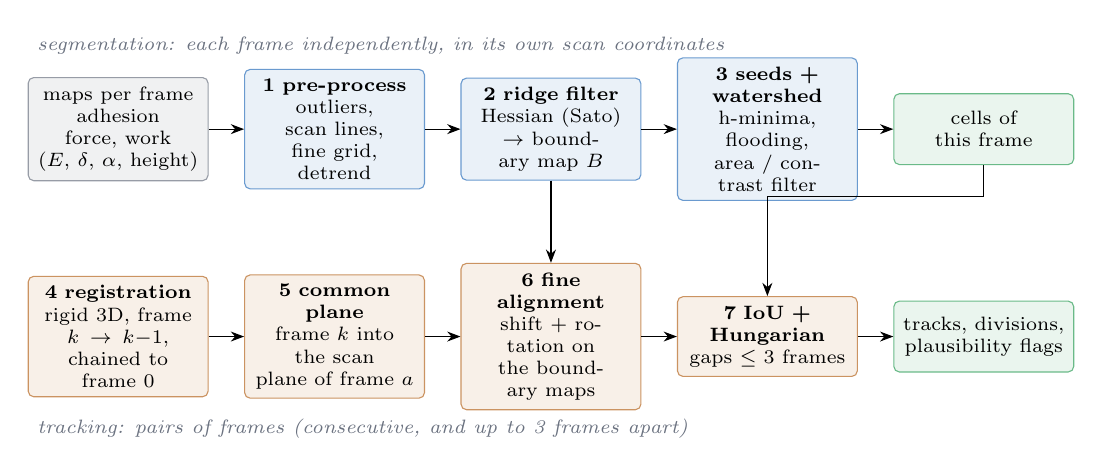
\begin{tikzpicture}[node distance=4mm and 4.5mm,>=Stealth]
\node[box=cGrey] (in) {maps per frame\\adhesion force, work\\($E$, $\delta$, $\alpha$, height)};
\node[box,right=of in] (pre) {\textbf{1 pre-process}\\outliers, scan lines,\\fine grid, detrend};
\node[box,right=of pre] (rid) {\textbf{2 ridge filter}\\Hessian (Sato)\\$\to$ boundary map $B$};
\node[box,right=of rid] (ws) {\textbf{3 seeds + watershed}\\h-minima, flooding,\\area / contrast filter};
\node[box=cGreen,right=of ws] (lab) {cells of\\this frame};
\node[box=cOrange,below=12mm of in] (reg) {\textbf{4 registration}\\rigid 3D, frame $k\to k{-}1$,\\chained to frame 0};
\node[box=cOrange,right=of reg] (pl) {\textbf{5 common plane}\\frame $k$ into the scan\\plane of frame $a$};
\node[box=cOrange,right=of pl] (fa) {\textbf{6 fine alignment}\\shift + rotation on\\the boundary maps};
\node[box=cOrange,right=of fa] (iou) {\textbf{7 IoU + Hungarian}\\gaps $\le 3$ frames};
\node[box=cGreen,right=of iou] (tr) {tracks, divisions,\\plausibility flags};
\draw[->] (in)--(pre); \draw[->] (pre)--(rid); \draw[->] (rid)--(ws); \draw[->] (ws)--(lab);
\draw[->] (reg)--(pl); \draw[->] (pl)--(fa); \draw[->] (fa)--(iou); \draw[->] (iou)--(tr);
\draw[->] (lab.south) -- ++(0,-4mm) -| (iou.north);
\draw[->] (rid.south) -- ++(0,-2.5mm) -| (fa.north);
\node[font=\scriptsize\itshape,cGrey,anchor=west] at ($(in.north west)+(0,4mm)$) {segmentation: each frame independently, in its own scan coordinates};
\node[font=\scriptsize\itshape,cGrey,anchor=west] at ($(reg.south west)+(0,-4mm)$) {tracking: pairs of frames (consecutive, and up to 3 frames apart)};
\end{tikzpicture}
\end{frame}

% ===========================================================================
\section{Segmentation}

\begin{frame}{Input maps (frame 19:00:35)}
\centering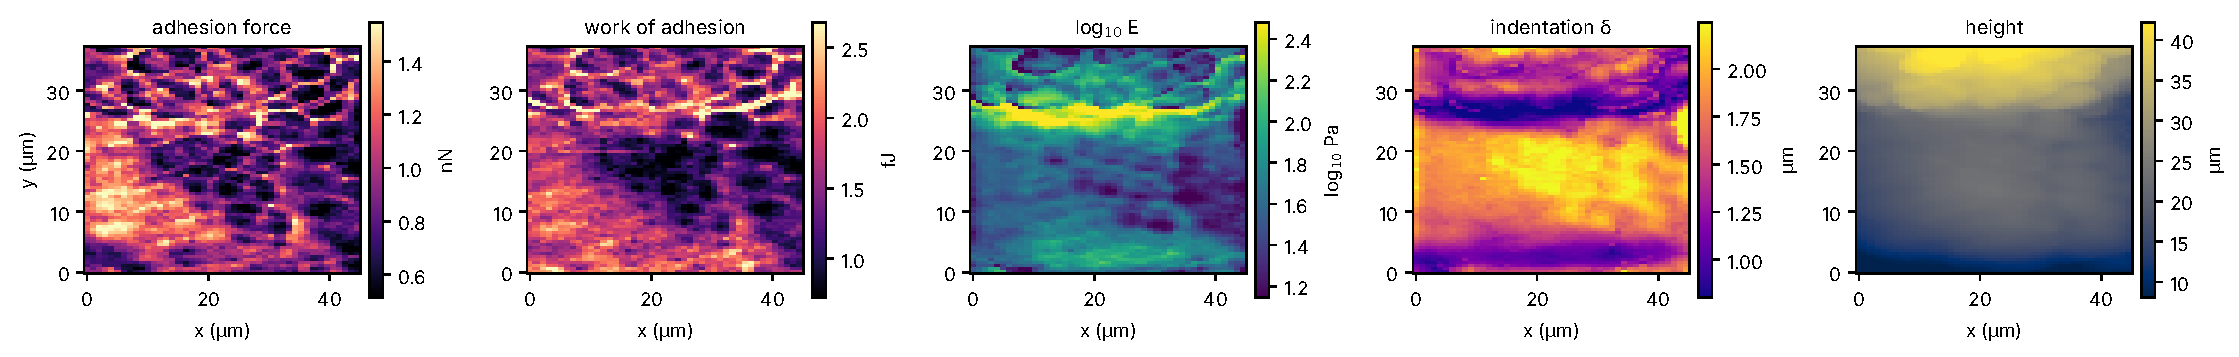
\includegraphics[width=\textwidth]{fig/channels.pdf}
\small
\begin{itemize}
\item In the \textbf{adhesion force} and \textbf{work of adhesion} maps the cell junctions are thin bright lines around dark cell interiors (a honeycomb, about 4\um{} per cell). These two maps are the default input.
\item $E$ and $\delta$ mainly show tissue-scale structure (the bright band at $y\approx\SI{27}{\micro\metre}$). The height map is smooth because the \SI{3}{\micro\metre} bead averages over a cell. They can be added with \texttt{--channels all}.
\item Polarity of a junction in each map: bright in adhesion force and work and in $E$, dark in $\delta$ and height. For $\alpha$ and the pull-off distance the sign is not known and is taken from the agreement with the other maps.
\end{itemize}
\end{frame}

\begin{frame}{All length scales follow one number: the cell diameter $D$}
\small
\begin{tabularx}{\textwidth}{@{}l l l X@{}}
\toprule
quantity & rule & $D=\SI{4}{\micro\metre}$ & role\\
\midrule
fine grid $h$ & $\min(D/16,\ p_x/2,\ p_y/2)$ & \SI{0.25}{\micro\metre} & all filtering and the watershed run on this isotropic grid\\
detrending scale & $D$ & \SI{4}{\micro\metre} & removes structure larger than a cell (tissue gradients)\\
ridge scales $\sigma_1,\sigma_2$ & $0.08D,\ 0.18D$ & \SI{0.32}{}, \SI{0.72}{\micro\metre} & widths of junction lines the filter responds to\\
smoothing of $B$ & $0.09D$ & \SI{0.36}{\micro\metre} & suppresses seeds from noise\\
minimum cell area & $0.15D^2$ & \SI{2.4}{\micro\metre\squared} & smaller regions are dropped\\
max.\ centroid step & $0.75D$ & \SI{3.0}{\micro\metre} & plausibility of a link between two observations\\
fine-alignment range & $\pm0.75D$ & $\pm\SI{3.0}{\micro\metre}$ & search range for the shift between two frames\\
\midrule
seed depth $h_\text{min}$ & -- & 0.1 & robust units (dimensionless)\\
boundary contrast & -- & 0.2 & robust units\\
outlier limit $K$ & -- & 4 & robust standard deviations\\
\bottomrule
\end{tabularx}\\[6pt]
Every map is converted to \emph{robust units} (median 0, robust SD 1) before thresholds are applied, so the thresholds do not depend on the unit or range of the map.
For another tissue, only $D$ (and the pixel size) has to be set; each scale can still be overridden (\texttt{--h}, \texttt{--ridge-um}, \dots).
\end{frame}

\begin{frame}{Step 1: pre-processing, the math}
\small
For each channel $A_{ij}$ (row $i$ = scan line, column $j$; $\log_{10}$ for $E$); $\Omega$ = pixels with data:
\begin{enumerate}
\item \textbf{Isolated-outlier filter.} $N_{ij}$ = the 8 neighbours, $m_{ij}=\med N_{ij}$, $r_{ij}=A_{ij}-m_{ij}$, $s=1.4826\,\med_{\Omega}|r_{ij}|$.\\
With $n^{(2)}_\uparrow$, $n^{(2)}_\downarrow$ = 2nd highest and 2nd lowest neighbour:
\[ A_{ij}\ \text{is an outlier}\iff A_{ij}-n^{(2)}_\uparrow>K s\ \ \text{or}\ \ n^{(2)}_\downarrow-A_{ij}>K s\qquad(K=4)\ \Rightarrow\ A_{ij}\leftarrow m_{ij}\]
A single-pixel spike differs from at least 7 of its 8 neighbours. A pixel on a junction line has $\ge2$ similar neighbours along the line, so it is \emph{not} removed.
\item \textbf{Scan-line offsets} (each line has its own baseline): $o_i=\med_j\bigl[A_{ij}-\med_{|i'-i|\le3}A_{i'j}\bigr]$, then $A_{ij}\leftarrow A_{ij}-o_i$.
\item \textbf{Fine isotropic grid}: cubic-spline resampling from $p_x\times p_y$ to $h\times h$ (here 45$\times$75 $\to$ 182$\times$150 points).
\item \textbf{Equal resolution in $x$ and $y$}: the fast axis is sampled twice as coarsely ($p_x\approx2p_y$). A Gaussian with $\sigma_y=\max(0.8,\ 0.6\,p_x/h)\,h=\SI{0.61}{\micro\metre}$ (and $\sigma_x=0.3h$) blurs $y$ to match $x$.
\item \textbf{Detrend and normalise}: $X\leftarrow X-G_{D}*X$ ($G_D$ = Gaussian, $\sigma=D$), then $z=(X-\med X)/(1.4826\MAD X)$.
\end{enumerate}
Masked holes: if a channel has holes, it is not used within \SI{1}{\micro\metre} of a hole edge (the filling there is not data).
\end{frame}

\begin{frame}{Step 1: example (adhesion force, 19:00:35)}
\centering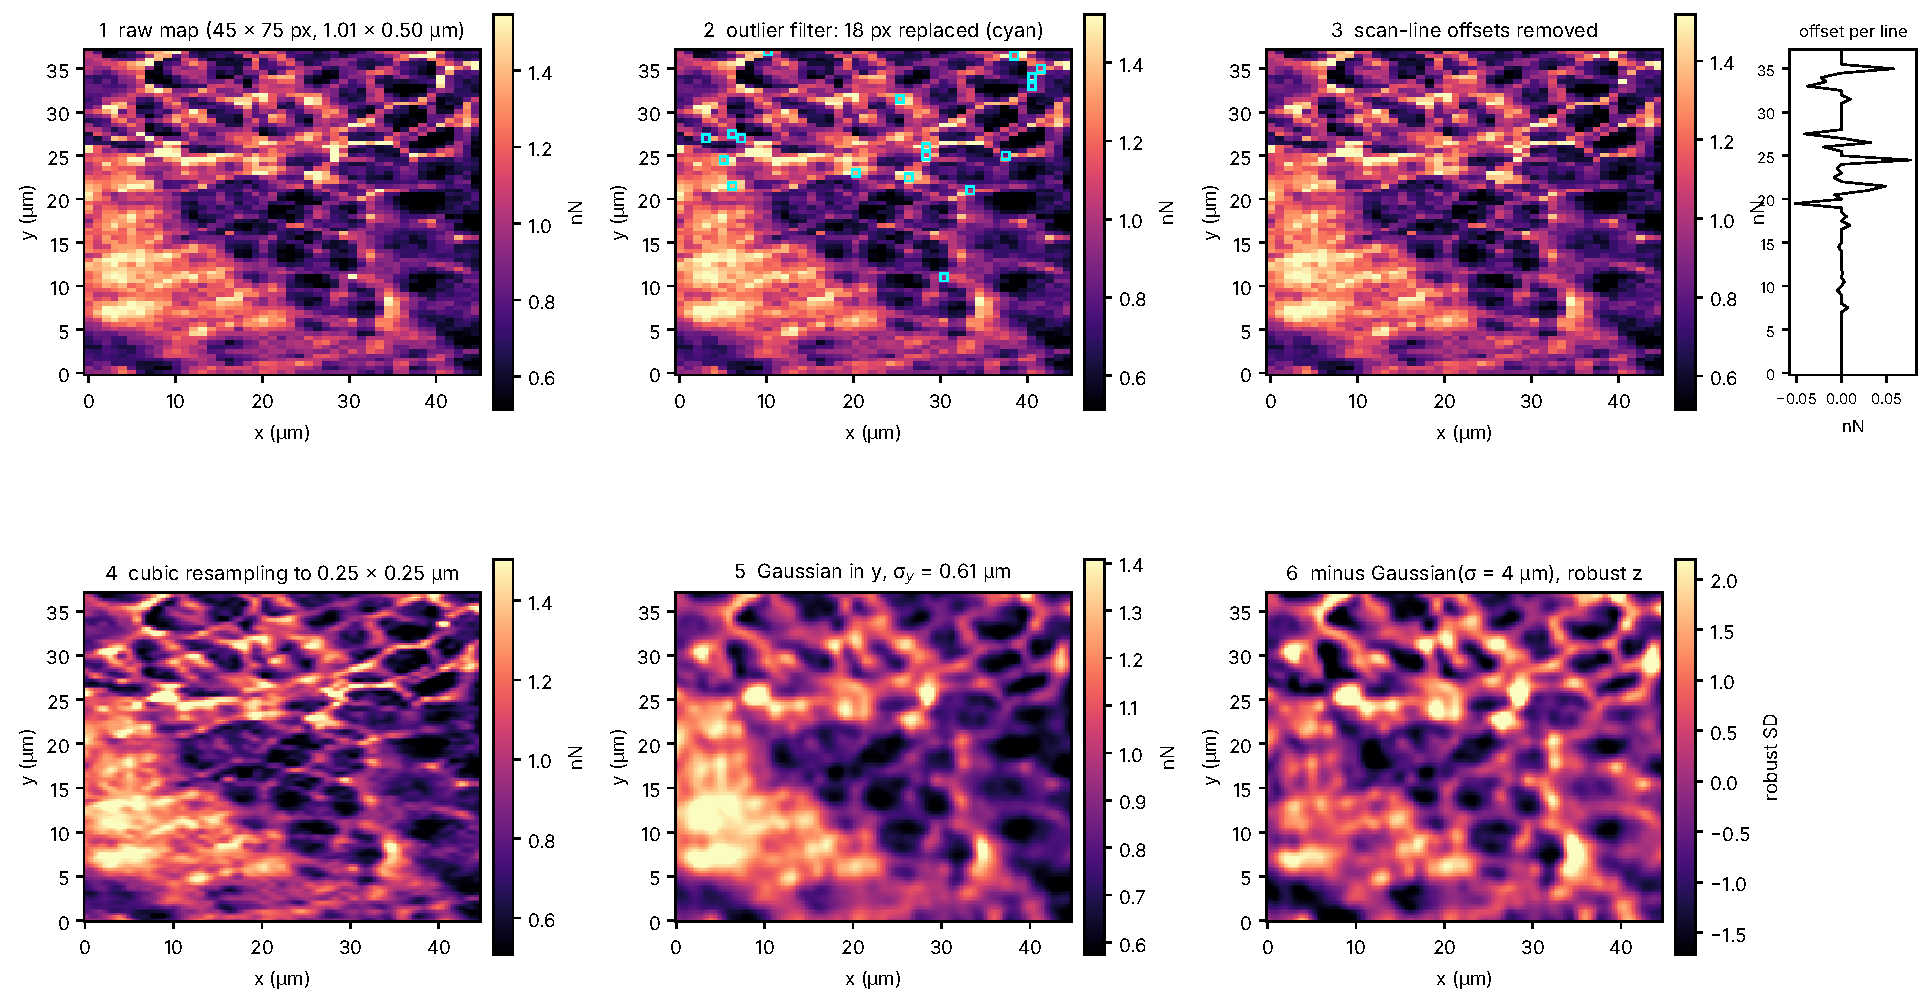
\includegraphics[height=0.80\textheight]{fig/preprocess.pdf}\\
\scriptsize 18 isolated outliers replaced (cyan). The scan-line offsets are small here (inset), $\lesssim\SI{0.05}{\nano\newton}$. Panel 6 is the input of the ridge filter.
\end{frame}

\begin{frame}{Step 2: junctions as ridges, the math}
\small
A junction is a thin line that is brighter than its surroundings. Across the line the intensity has a sharp maximum, so the second derivative is strongly negative; along the line it is $\approx0$.\\[4pt]
\textbf{Hessian at scale $\sigma$} (Gaussian derivatives):
\[\mathbf H_\sigma(\mathbf x)=\begin{pmatrix}\partial_{xx}&\partial_{xy}\\ \partial_{xy}&\partial_{yy}\end{pmatrix}(G_\sigma*z)(\mathbf x),\qquad \text{eigenvalues }\lambda_{\min}\le\lambda_{\max}\]
\textbf{Sato line filter} for bright ridges (for dark ridges, e.g.\ $\delta$, use $-z$):
\[R(\mathbf x)=\max_{\sigma\in\{\sigma_1,\sigma_2\}}\ \sigma^2\max\bigl(-\lambda_{\min}(\mathbf x;\sigma),\,0\bigr),\qquad \sigma_1=\SI{0.32}{\micro\metre},\ \sigma_2=\SI{0.72}{\micro\metre}\]
\begin{itemize}
\item $-\lambda_{\min}$ is the curvature across the line. It does not depend on the line direction, so junctions in every direction respond the same way.
\item The factor $\sigma^2$ makes the two scales comparable (scale normalisation).
\item Smooth gradients have $\lambda\approx0$ and give no response. A bright spot gives a response too, but the watershed only needs \emph{where} the barriers are.
\end{itemize}
Each channel's $R$ is converted to robust units: $\tilde R_n=(R_n-\med R_n)/(1.4826\MAD R_n)$.
\end{frame}

\begin{frame}{Step 2: example, one line across the map}
\begin{columns}[T]
\begin{column}{0.58\textwidth}
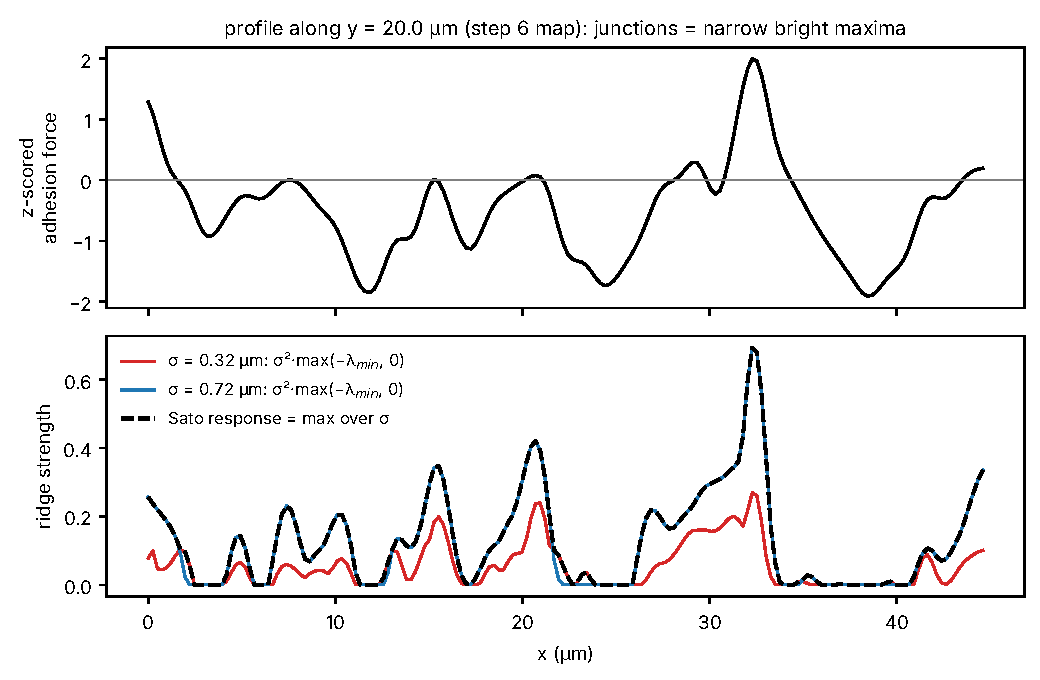
\includegraphics[width=\textwidth]{fig/ridge1d.pdf}
\end{column}
\begin{column}{0.40\textwidth}\small
\begin{itemize}
\item Top: z-scored adhesion force along $y=\SI{20}{\micro\metre}$ (panel 6 of the previous example). Each narrow maximum is a junction, each wide minimum a cell interior.
\item Bottom: $\sigma^2\max(-\lambda_{\min},0)$ at both scales, and their maximum (Sato response).
\item The cell interiors give 0, so they become the basins of the watershed.
\item The small scale (red) separates junctions that lie close together. The large scale (blue) picks up broad or weak junctions.
\end{itemize}
\end{column}
\end{columns}
\end{frame}

\begin{frame}{Step 2: combining the channels into one boundary map $B$}
\centering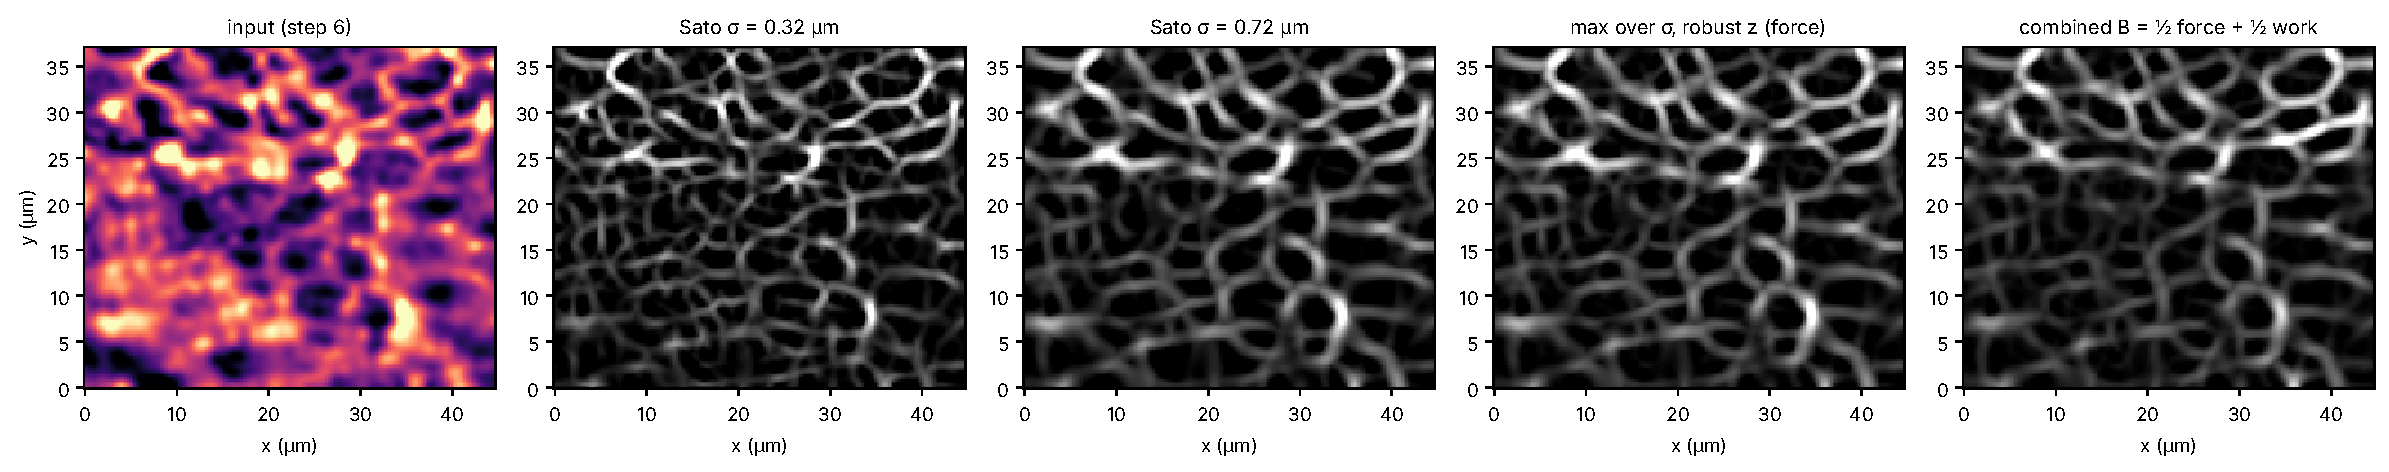
\includegraphics[width=\textwidth]{fig/ridge2d.pdf}
\small
\[w_n=\frac{\max\bigl(0,\ \rho(\tilde R_n,\ \overline{\tilde R}_{m\ne n})\bigr)}{\sum_k\max(0,\rho(\cdot))},\qquad
B(\mathbf x)=\frac{\sum_n w_n\,M_n(\mathbf x)\,\tilde R_n(\mathbf x)}{\sum_n w_n\,M_n(\mathbf x)}\ \ \text{where }\textstyle\sum_n w_nM_n>0.25\]
$\rho$ = Pearson correlation with the mean of the other channels, $M_n$ = 1 where channel $n$ has data. A channel that does not agree with the others gets weight 0. The height map is capped at $w\le0.2$ (the bead blurs it).
With the two default channels, $\rho$ is symmetric, so $w=\tfrac12,\tfrac12$.
\end{frame}

\begin{frame}{Step 3: seeds = basins of at least depth $h$ (h-minima)}
\begin{columns}[T]
\begin{column}{0.56\textwidth}
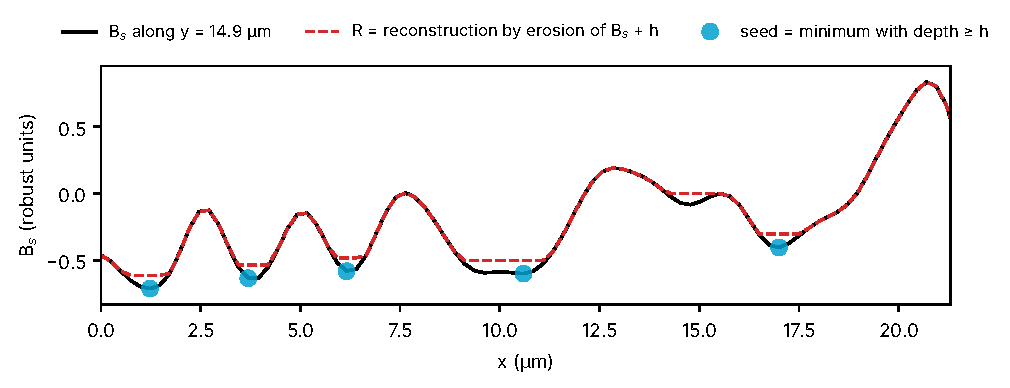
\includegraphics[width=\textwidth]{fig/hmin1d.pdf}\\
\scriptsize 1D illustration on a real line of $B_s$ ($h=0.1$). In the maps the same is done in 2D.
\end{column}
\begin{column}{0.42\textwidth}\small
$B_s=G_{0.09D}*B$ (smoothed boundary map).\\[3pt]
\textbf{Reconstruction by erosion}: start from $B_s+h$ and erode repeatedly, never below $B_s$:
\[\mathcal R=\rho^{\varepsilon}\bigl(B_s+h\ \big|\ B_s\bigr)\]
Basins shallower than $h$ are filled up to their spill level. Deeper basins keep a ``lid'' exactly $h$ above their bottom.
\[\text{seeds}=\{\mathbf x:\ \mathcal R(\mathbf x)-B_s(\mathbf x)\ge h\}\]
These are the regional minima whose \emph{dynamic} (depth to the lowest pass) is $\ge h$, labelled as connected components.\\[3pt]
Dashed: $\mathcal R$. The dip at $x\approx\SI{14.5}{\micro\metre}$ is shallower than $h$, so it gets no seed and becomes part of a neighbouring cell.
\end{column}
\end{columns}
\end{frame}

\begin{frame}{Step 3: watershed, filters and result (19:00:35)}
\centering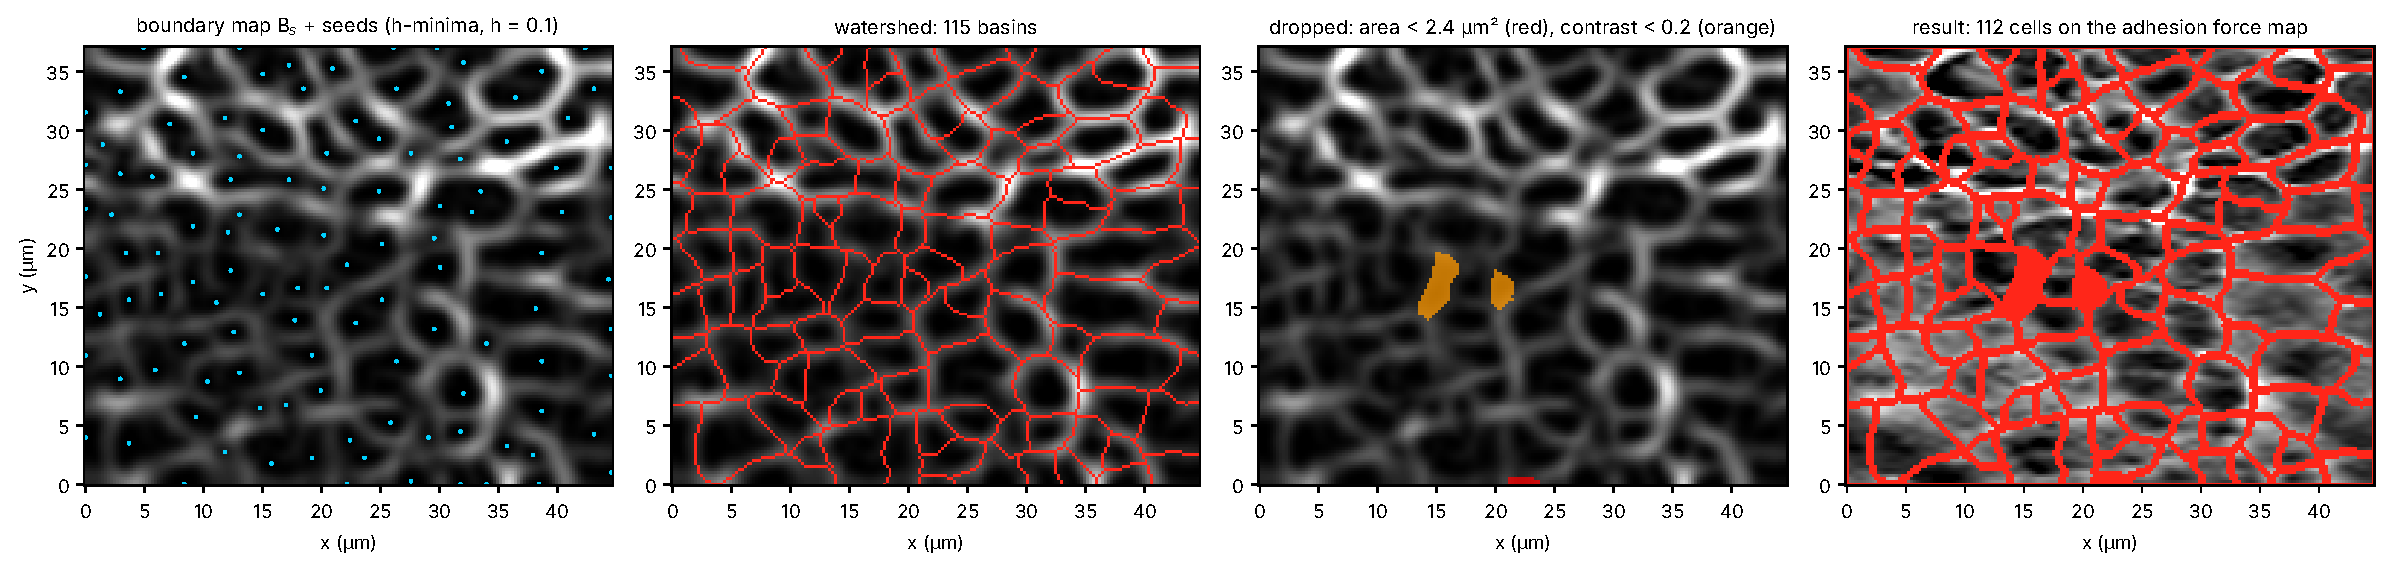
\includegraphics[width=\textwidth]{fig/watershed.pdf}
\small
\begin{columns}[T]
\begin{column}{0.5\textwidth}
\textbf{Watershed}: flood $B_s$ from the seeds in order of increasing $B_s$. Each pixel joins the basin that reaches it first; where two basins meet, a 1-pixel line (label 0) is left. Here: 115 seeds $\to$ 115 basins.
\end{column}
\begin{column}{0.48\textwidth}
\textbf{Keep a basin $c$ only if}
\begin{itemize}
\item area $\ge0.15D^2=\SI{2.4}{\micro\metre\squared}$ (1 dropped, \SI{1.9}{\micro\metre\squared})
\item contrast $\med_{\text{ring}}B_s-\med_{c}B_s\ge0.2$, ring = 2 pixels around $c$ (2 dropped: 0.18 and 0.18). This drops regions without a closed junction.
\end{itemize}
$\Rightarrow$ \textbf{112 cells}.
\end{column}
\end{columns}
\end{frame}

\begin{frame}{Outputs per cell}
\small
\begin{itemize}
\item Labels on the fine grid are saved as \texttt{cells\_hr}. Each measured pixel gets the label of the nearest fine-grid point (\texttt{cells}).
\item Per cell and frame (\texttt{cells\_table.csv}), with $g_x,g_y$ = height gradient:
\[A_\text{proj}=n_\text{px}\,p_xp_y,\qquad A_\text{surf}=\sum_{\text{px}\in c}p_xp_y\sqrt{1+g_x^2+g_y^2},\qquad d_\text{eq}=\sqrt{4A_\text{surf}/\pi}\]
\item Further columns:
 \begin{itemize}
 \item 3D centroid in registered coordinates and in the frame's own coordinates;
 \item median slope;
 \item boundary contrast;
 \item $E$ at the junctions (1-pixel ring) and at the centre;
 \item axes, orientation, solidity and perimeter (from the fine grid);
 \item the median of every map.
 \end{itemize}
\item Median over all 4385 cells: $A_\text{proj}=\SI{11.1}{\micro\metre\squared}$, $A_\text{surf}=\SI{16.6}{\micro\metre\squared}$ (the surface is tilted and curved), $d_\text{eq}=\SI{4.6}{\micro\metre}$.
\end{itemize}
\end{frame}

\begin{frame}{Before vs.\ now: why the cells came out about twice too large}
\begin{columns}[T]
\begin{column}{0.56\textwidth}
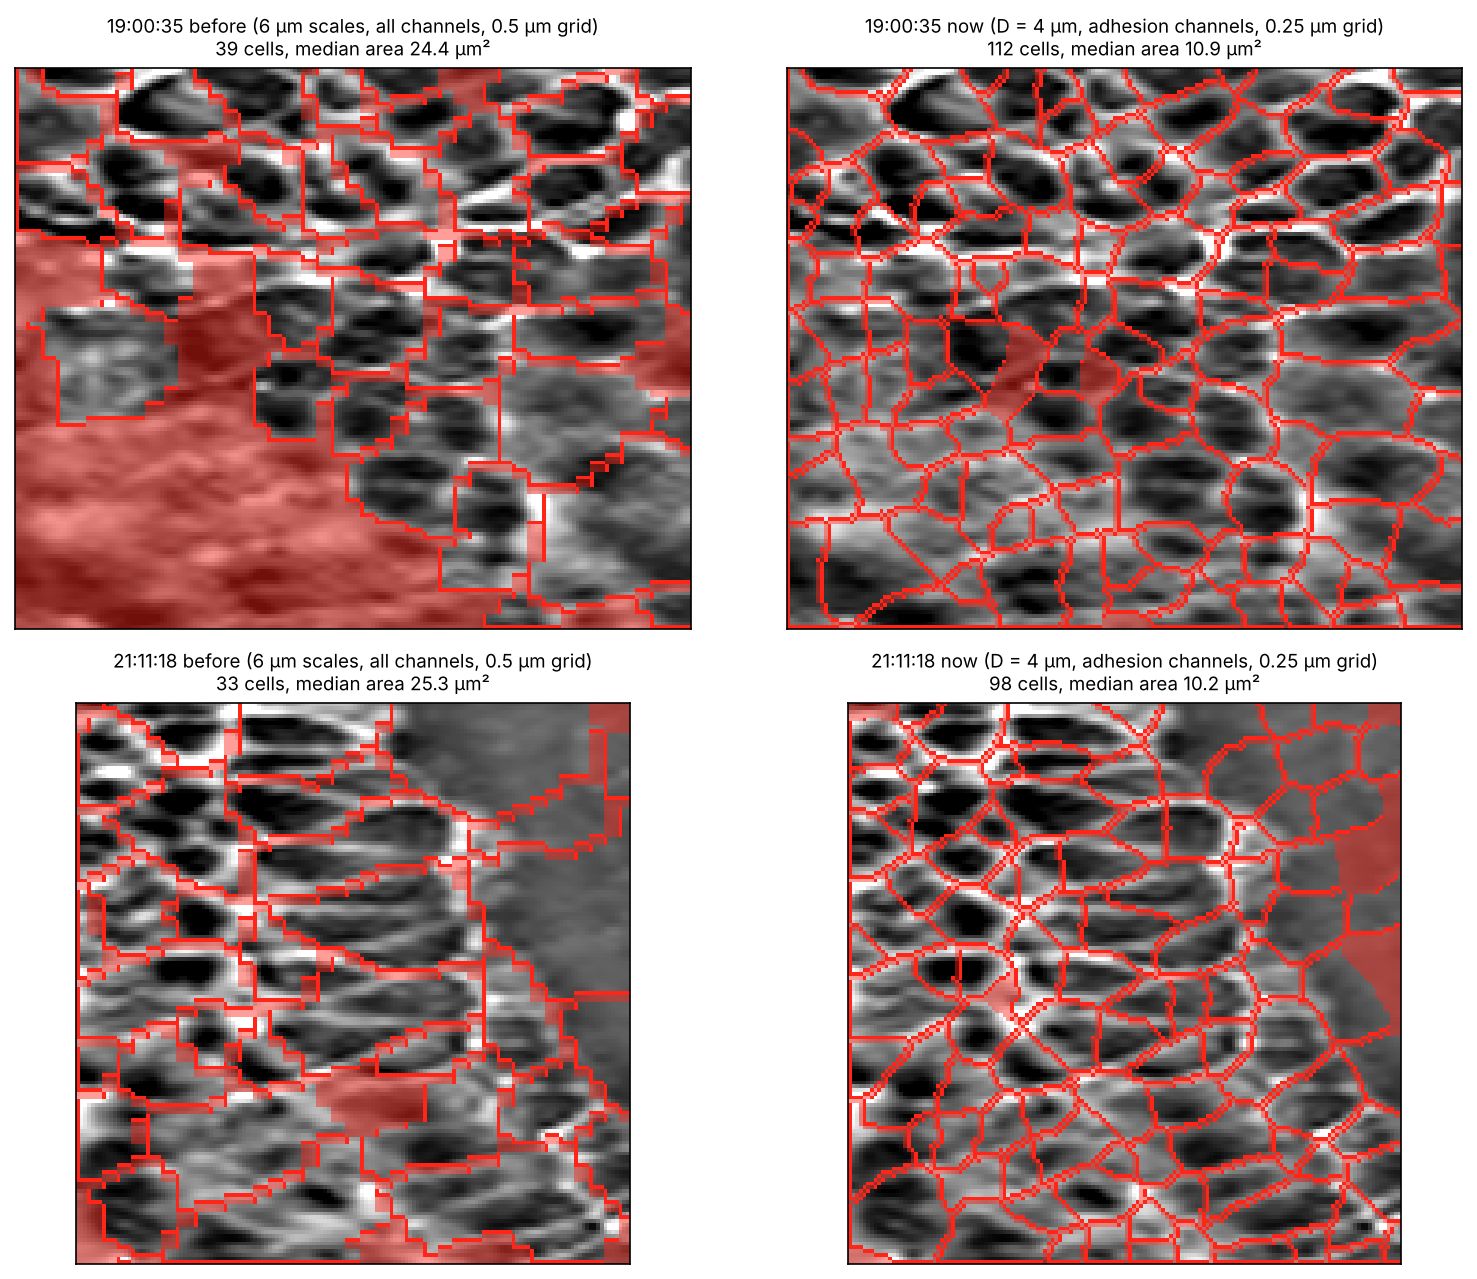
\includegraphics[height=0.84\textheight]{fig/oldnew.png}
\end{column}
\begin{column}{0.42\textwidth}\small
\textbf{Before}:
\begin{itemize}
\item scales set for $\approx\SI{6}{\micro\metre}$ cells: detrending \SI{6}{\micro\metre}, ridges 0.5--\SI{1}{\micro\metre}, seed depth 0.35, minimum area \SI{6}{\micro\metre\squared};
\item all channels, on a \SI{0.5}{\micro\metre} grid.
\end{itemize}
Shallow basins were merged, so most regions held two cells, and large areas stayed unsegmented. Median \SI{24}{\micro\metre\squared}.\\[4pt]
\textbf{Now}:
\begin{itemize}
\item $D=\SI{4}{\micro\metre}$, seed depth 0.1;
\item the adhesion channels only (their junction contrast is the sharpest);
\item a \SI{0.25}{\micro\metre} grid with cubic resampling.
\end{itemize}
Median \SI{11}{\micro\metre\squared}. About one dark cell interior per region, as seen on the maps; 2.4$\times$ more cells per frame (102 vs.\ 42, median).\\[4pt]
\scriptsize Red shading = unsegmented (label 0).
\end{column}
\end{columns}
\end{frame}

% ===========================================================================
\section{Tracking}

\begin{frame}{Step 4: rigid 3D registration of consecutive frames}
\small
The embryo moves and rolls under the probe. Frame $k$ is registered onto frame $k-1$ with a \textbf{rigid} transform (no scaling) $\mathbf q=\mathbf R\mathbf p+\mathbf t$, with $\mathbf p=(x,y,z)$ in the scan coordinates of frame $k$ and $z$ = height.
\begin{enumerate}
\item \textbf{Start}: rotation $\theta$ about the vertical axis plus shift.
 \begin{itemize}
 \item grid search: $\theta\in[-24^\circ,24^\circ]$ in $3^\circ$ steps, shifts $\pm\SI{24}{\micro\metre}$ in \SI{2}{\micro\metre} steps;
 \item cost: Huber loss ($\delta=\SI{1}{\micro\metre}$) of the height differences after removing their median, plus $0.02\,(1-\text{overlap})$;
 \item refined with Nelder--Mead.
 \end{itemize}
\item \textbf{Full 3D}: 7 parameters, the rotation vector $\bm\omega$ ($\mathbf R=\exp[\bm\omega]_\times$), $\mathbf t$ and a log-$E$ offset $c$. Residuals per point:
\[r_z=\frac{z_{k-1}(q_x,q_y)-q_z}{\sqrt{1+|\nabla z_{k-1}|^2}}\ \ (\approx\text{normal distance}),\qquad r_E=\SI{3}{\micro\metre}\cdot\bigl(\log E_{k-1}(\mathbf q)-\log E_k(\mathbf p)-c\bigr)\]
 \begin{itemize}
 \item outside the overlap, $r=\SI{1}{\micro\metre}$;
 \item minimise $\sum\rho(r)$ with the robust loss $\rho(r)=2f^2(\sqrt{1+(r/f)^2}-1)$, $f=\SI{0.5}{\micro\metre}$;
 \item starts: the solution of step 1, and rotations about pivots \SI{6}{}, \SI{30}{} and \SI{90}{\micro\metre} below the surface (rolling). The best result is kept.
 \end{itemize}
\item \textbf{Chain}: with $\mathbf H_k$ = 4$\times$4 transform $k\to k-1$: $\mathbf G_0=\mathbf I$, $\mathbf G_k=\mathbf G_{k-1}\mathbf H_k$ maps frame $k$ into frame 0.
\end{enumerate}
Cached in \texttt{registration.json}; the viewer uses the same transforms.
\end{frame}

\begin{frame}{Step 5--6: compare two frames in one plane, then fine-align}
\begin{columns}[T]
\begin{column}{0.5\textwidth}\small
\textbf{Common plane.} Frame $k$ is compared with an earlier frame $a$ (normally $a=k-1$) in $a$'s own scan plane:
\[\mathbf G_{a\leftarrow k}=\mathbf G_a^{-1}\mathbf G_k,\qquad (x',y')=\bigl[\mathbf G_{a\leftarrow k}(x,y,z,1)^\top\bigr]_{1,2}\]
Projecting both onto frame 0 instead would shrink cells on surfaces tilted against frame 0 (the cumulative tilt reaches tens of degrees).\\[4pt]
\textbf{Fine alignment.} The registration fits the height (blurred by the bead). Cells need sub-cell precision, so a 2D rigid correction is fitted on the boundary maps:
\[\max_{\theta,\Delta x,\Delta y}\ \rho\bigl(B_a(\mathbf q),\,B_k(\mathbf p)\bigr),\quad \mathbf q=\mathbf R_\theta(\mathbf p-\mathbf c)+\mathbf c+\Delta\]
($\mathbf c$ = centroid). Grid search: $\pm4^\circ$ in $1^\circ$ steps and $\pm0.75D$ in \SI{0.5}{\micro\metre} steps, then Nelder--Mead.
\end{column}
\begin{column}{0.48\textwidth}
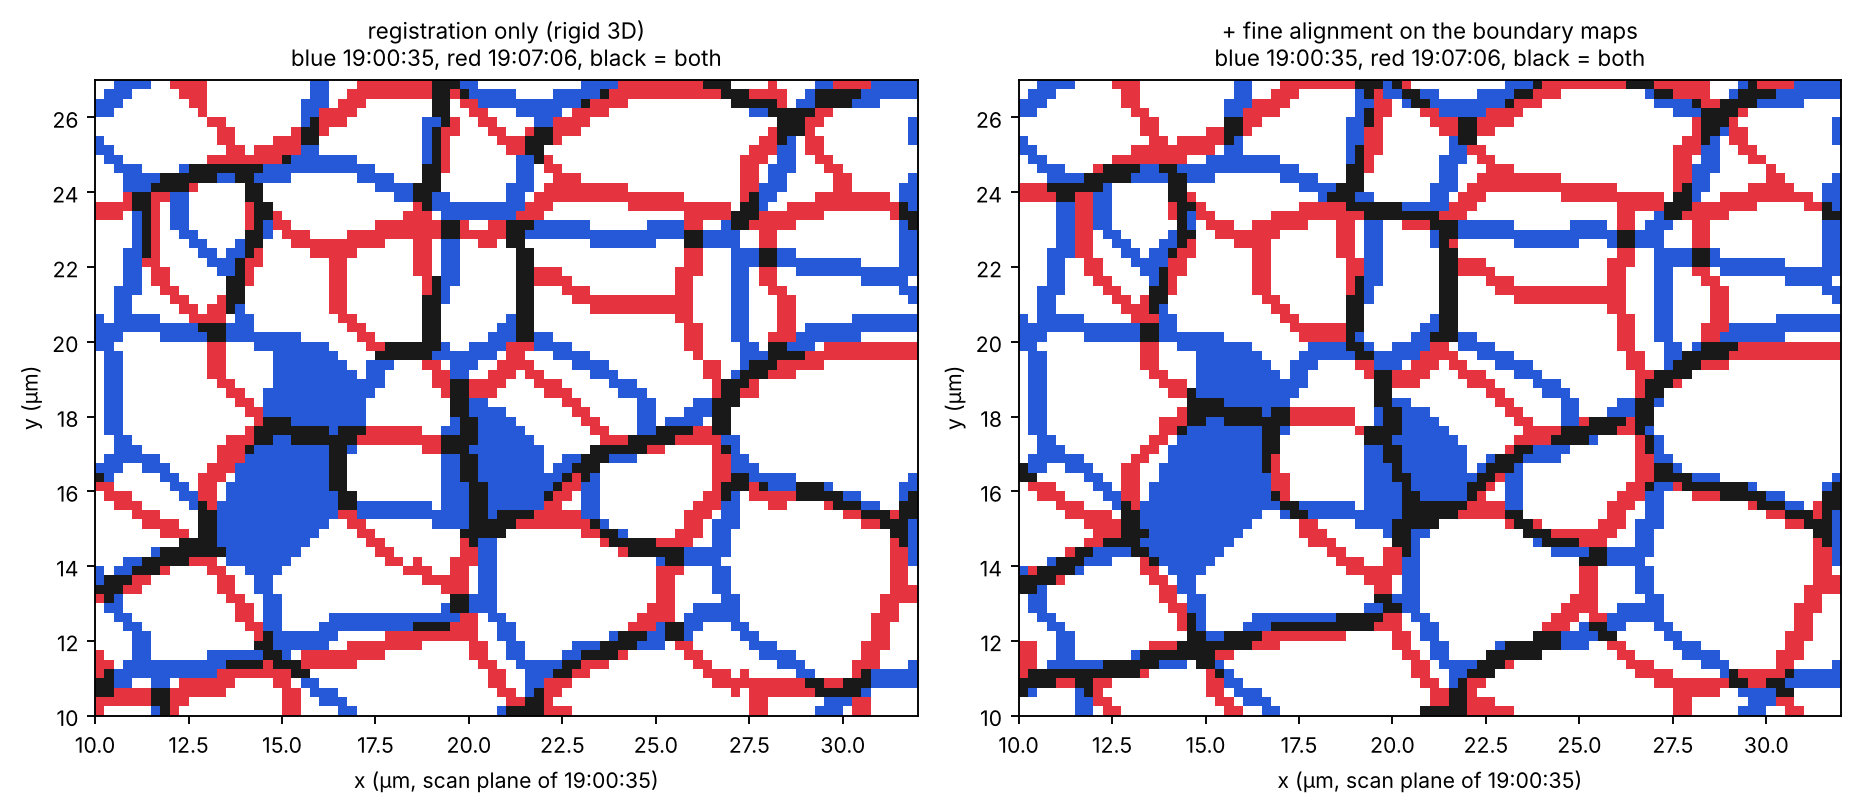
\includegraphics[width=\textwidth]{fig/align.png}\\
\scriptsize Example 19:00:35 $\leftarrow$ 19:07:06: relative motion $1.5^\circ$ and $(1.5,-0.8,-0.8)$\um. Fine alignment adds $-0.7^\circ$ and $(0.10,0.27)$\um; correlation $0.41\to0.44$. Over all consecutive pairs (median): correlation $0.50\to0.53$, \SI{0.36}{\micro\metre}, $0.8^\circ$. Solid blue = unsegmented area. Many junctions coincide (black). Others do not: the segmentation is not identical from frame to frame.
\end{column}
\end{columns}
\end{frame}

\begin{frame}{Step 7: overlap (IoU) and optimal one-to-one assignment}
\begin{columns}[T]
\begin{column}{0.5\textwidth}\small
Every pixel of both frames is assigned to a bin of $a$'s pixel grid: $\mathbf b=\bigl(\lfloor x'/p_x+\tfrac12\rfloor,\lfloor y'/p_y+\tfrac12\rfloor\bigr)$. A cell is then a set of bins, $S_c$.
\[\IoU(c,d)=\frac{|S_c\cap S_d|}{|S_c|+|S_d|-|S_c\cap S_d|}\in[0,1]\]
\textbf{Assignment} (Hungarian algorithm): choose a one-to-one matching $\pi$ between cells of $a$ and cells of $k$ that maximises
\[\sum_c \IoU\bigl(c,\pi(c)\bigr)\]
Keep only links with $\IoU\ge0.2$. One cell cannot be linked to two cells, and the best \emph{global} matching wins over greedy choices.\\[4pt]
Example: 112 cells (19:00:35) and 103 cells (19:07:06) give 82 direct links, median IoU 0.42.
\end{column}
\begin{column}{0.48\textwidth}
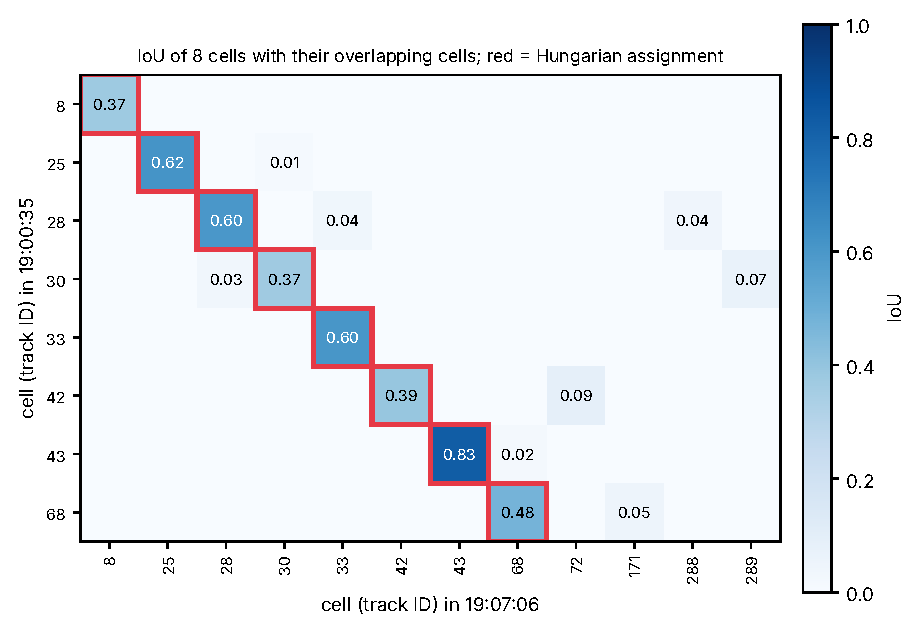
\includegraphics[width=\textwidth]{fig/iou.pdf}
\end{column}
\end{columns}
\end{frame}

\begin{frame}{Gaps, new tracks, divisions}
\small
\textbf{Gap bridging} (a cell missed in a frame, e.g.\ merged or not segmented): for frame $k$ and $g=1,\dots,4$:
\begin{itemize}
\item candidates are the tracks whose last observation was frame $k-g$, and the cells of $k$ not yet linked;
\item same IoU and Hungarian step as above, in the scan plane of $k-g$ with its own fine alignment.
\end{itemize}
The nearest frame comes first; up to 3 missing frames are bridged. In this data, 269 links cross a gap.\\[4pt]
\textbf{New track}: every cell of $k$ that is still unlinked.\\[4pt]
\textbf{Division candidate}: new cell $b$ and the linked successor $b_1$ of a cell $a$ of frame $k-1$ with
\[\frac{|S_a\cap S_b|}{|S_b|}\ge0.5,\quad\frac{|S_a\cap S_{b_1}|}{|S_{b_1}|}\ge0.5,\quad 0.6\le\frac{|S_b|+|S_{b_1}|}{|S_a|}\le1.5,\quad 0.2\le\frac{|S_b|}{|S_a|}\le0.8\]
i.e.\ both lie mostly inside the old cell and together have about its area. $b$ gets parent = track of $a$.\\
\textbf{``confirmed''}: the daughter is observed in $\ge3$ frames and the mother continues for $\ge2$ frames after the split.
\end{frame}

\begin{frame}{Division example, and how far to trust it}
\centering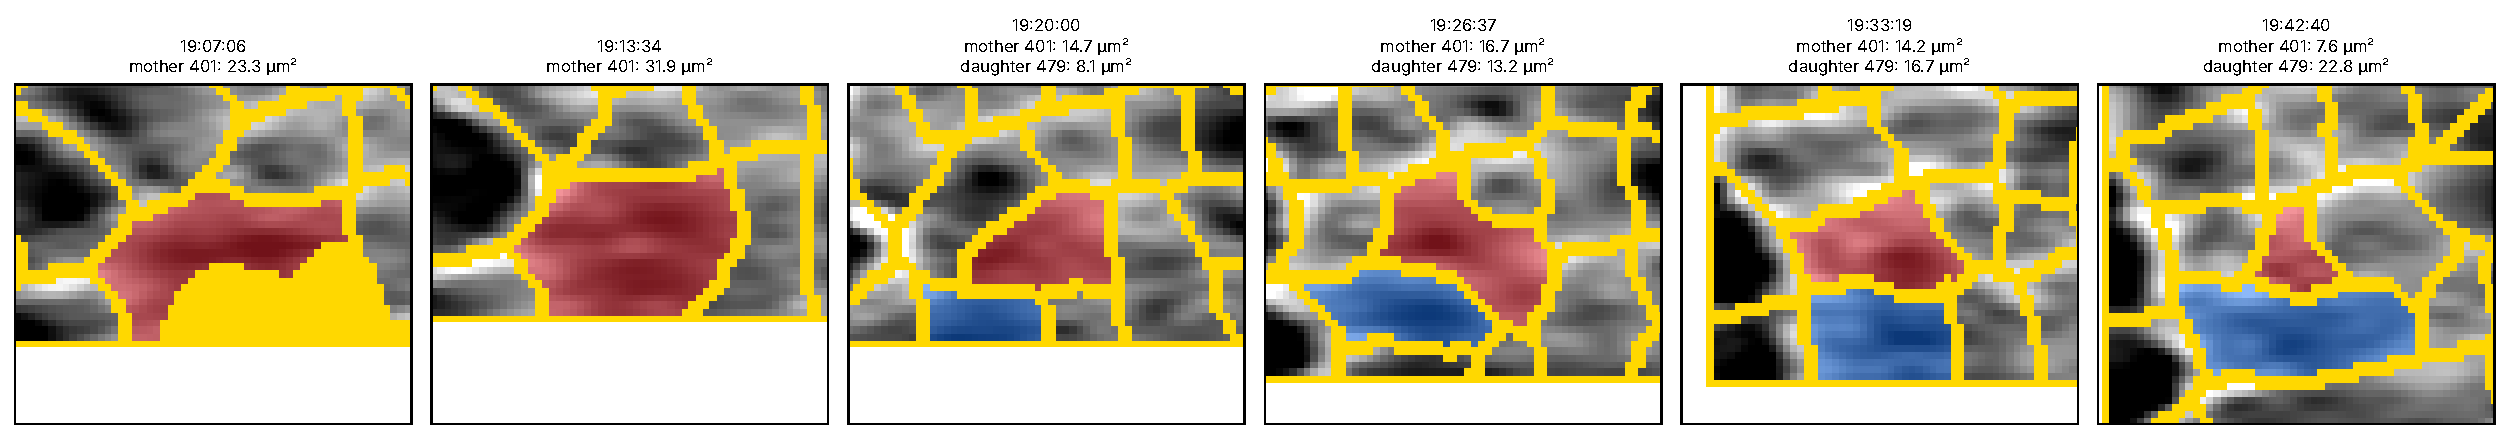
\includegraphics[width=\textwidth]{fig/division.pdf}
\small
\begin{itemize}
\item Mother 401 (red, 31.9\,\si{\micro\metre\squared} at 19:13:34) $\to$ mother 14.7 + daughter 479 (blue) 8.1\,\si{\micro\metre\squared} at 19:20:00. Both persist in the following frames.
\item Over the whole data set: 74 ``confirmed'' and 123 candidates. Only 28 of the 74 have both cells present in $\ge5$ of the 6 following frames.
\item AFM sees neither nuclei nor a cleavage furrow, and a cell that is split in one frame and merged in the next (segmentation flicker) also meets the criteria. Treat these as \textbf{candidates}, to be checked against the maps or the viewer, not as proven divisions.
\end{itemize}
\end{frame}

\begin{frame}{Plausibility of every link}
\centering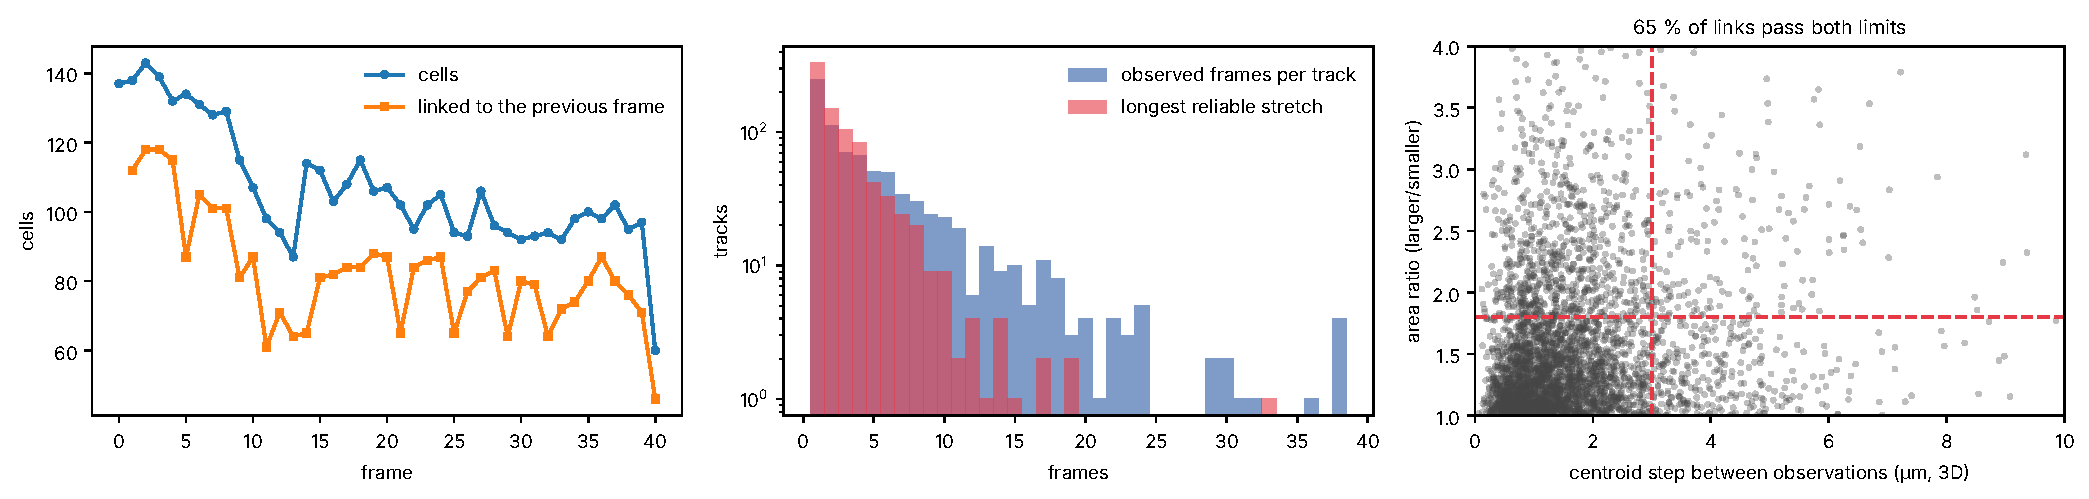
\includegraphics[width=\textwidth]{fig/trackstats.pdf}
\small
For consecutive observations of a track:
\begin{itemize}
\item step $=\|\mathbf x_\text{reg}(t_2)-\mathbf x_\text{reg}(t_1)\|$ (registered 3D centroid);
\item area ratio $=\max(A_1,A_2)/\min(A_1,A_2)$ of $A_\text{surf}$.
\end{itemize}
A link is \texttt{link\_ok} if step $\le0.75D=\SI{3}{\micro\metre}$ and ratio $\le1.8$. Otherwise the track is cut into \texttt{reliable\_segment}s.\\
Here 65\,\% of the links pass (median step \SI{1.4}{\micro\metre}, median area ratio 1.39). Left: cells per frame and how many are linked to the previous frame (78\,\% overall).
\end{frame}

\begin{frame}{Results for this data set}
\begin{columns}[T]
\begin{column}{0.44\textwidth}\scriptsize
\begin{tabular}{@{}lr@{}}
\toprule
cells per frame (median) & 102\\
cells in total & 4385\\
median area proj./surface (\si{\micro\metre\squared}) & 11.1/16.6\\
tracks & 823\\
tracks seen in $\ge$5/10/20/30 frames & 325/136/28/9\\
longest track & 38 of 41 frames\\
reliable stretch $\ge$5/10/15/20 & 154/26/6/1\\
longest reliable stretch & 33 frames\\
linked to the previous frame & 78\,\%\\
links passing both checks & 65\,\%\\
\bottomrule
\end{tabular}
\end{column}
\begin{column}{0.54\textwidth}
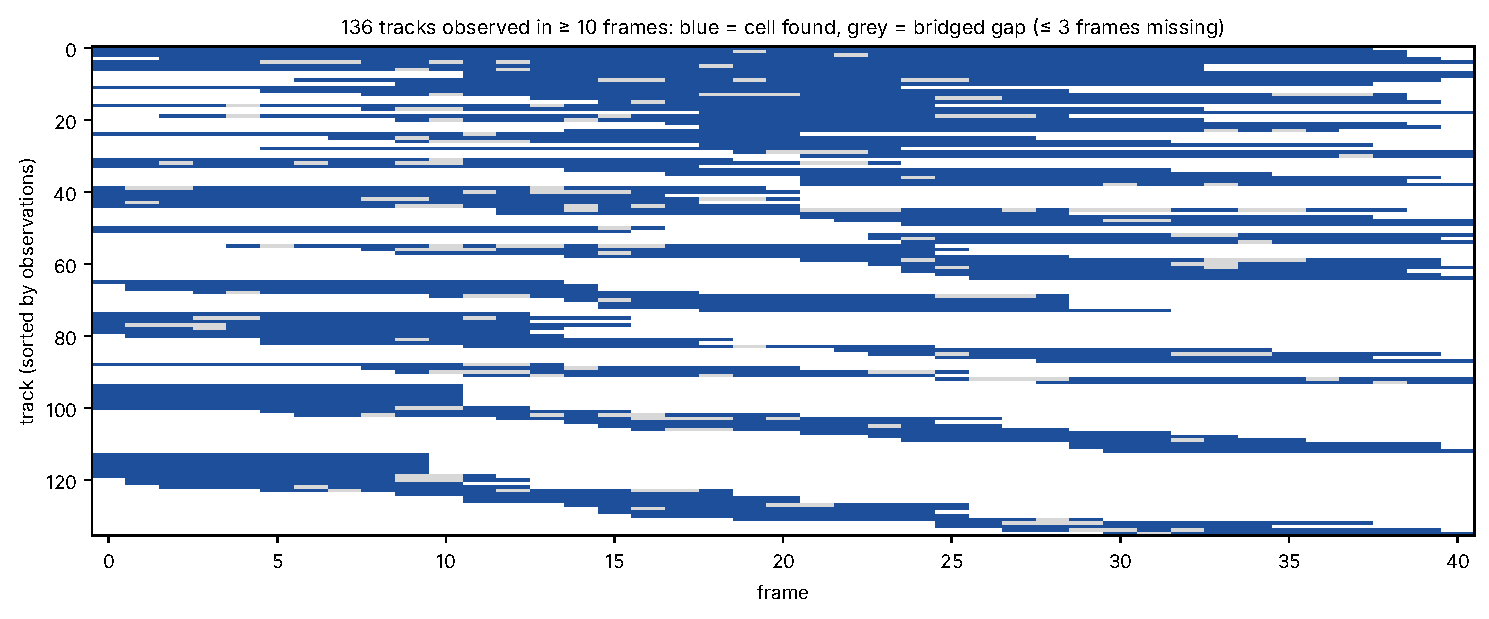
\includegraphics[width=\textwidth]{fig/lifelines.pdf}
\end{column}
\end{columns}
\vspace{4pt}\small
A ``reliable stretch'' is the longest run of consecutive links of a track that pass both plausibility checks. For analyses that need the same cell over time, use reliable stretches, not whole tracks.
\end{frame}

% ===========================================================================
\section{Viewer}

\begin{frame}{Viewer: sharper and smoother display, outliers, holes}
\small
\textbf{Display grid} (\emph{grid}: raw / \SI{0.5}{} / \SI{0.25}{\micro\metre}): every map is resampled to an isotropic grid with bicubic (Catmull--Rom) interpolation, using $\log_{10}$ for $E$. Near missing data it falls back to bilinear interpolation.
\begin{itemize}
\item Categorical maps (cells, detached flag, rupture counts) and maps that are empty by design (rupture position where there is none, tether = 0) use the nearest pixel.
\item Cells come from the fine \texttt{cells\_hr} labels, and the red vector outlines are traced on that grid.
\end{itemize}
\textbf{Outlier filter + fill small holes} (checkbox):
\begin{itemize}
\item the same isolated-outlier rule as in the segmentation, with $K=5$;
\item holes of $\le12$ pixels inside the scanned area are filled from their neighbours;
\item large missing areas stay empty.
\end{itemize}
\textbf{Display only}: no number in the CSV files, the segmentation or the maps is changed. Interpolation makes the picture smooth but adds no resolution. The information is still that of the $1.01\times\SI{0.5}{\micro\metre}$ pixels.
\end{frame}

\begin{frame}{Viewer: holes, and what ``darken excluded pixels'' does}
\small
\textbf{Holes found and fixed}:
\begin{itemize}
\item Height spikes ($>\SI{5}{\micro\metre}$ from the 3$\times$3 median; 1--75 pixels in 19 frames) used to be removed and left holes in the surface. They are now replaced by the median.
\item In the last frame (21:48:03) the scan was aborted: 16 lines are missing, and 4 lines before them jumped by $\approx$\,40--50\,\si{\micro\metre} (the tip lost the surface). These lines are now removed. The registration of that frame improved from $37^\circ$ to $7.6^\circ$ with 91\,\% overlap.
\item \emph{darken excluded pixels} (sidebar group ``Excluded fits''): draws pixels at 60\,\% brightness that the fit flagged as excluded (steep, low $R^2$, deep $\delta$, $\alpha$ at bound) but that are shown, so they can be told apart.
\end{itemize}
\end{frame}

% ===========================================================================
\section{Limits and other data sets}

\begin{frame}{Limits}
\small
\begin{itemize}
\item \textbf{Resolution}: \SI{1.01}{\micro\metre} pixels along $x$ for $\approx\SI{4}{\micro\metre}$ cells means about 4 pixels per cell diameter. Junctions closer than $\approx\SI{2}{\micro\metre}$ cannot be separated in $x$, and cell shapes come out elongated along $x$. Areas and positions are usable; orientation and aspect ratio are not reliable.
\item \textbf{Surface only}: cells are patches of the outer surface. A cell that sinks below the surface or is covered disappears.
\item \textbf{Texture-free regions} (e.g.\ the top right at 21:11) can be cut into large regions if weak ridges close up. Use the boundary contrast column to filter them.
\item \textbf{Frame-to-frame consistency}: the segmentation of two frames is not identical (junction contrast changes with contact and adhesion). This causes split/merge flicker, which in turn produces false gaps and division candidates.
\item \textbf{Registration}: rigid only. Local tissue deformation between frames ($\approx6$ min) is absorbed by the fine alignment only up to $\pm\SI{3}{\micro\metre}$ and $\pm4^\circ$.
\item \textbf{Parameters}: $D$, seed depth and contrast were chosen by eye on the adhesion maps of this data set. There is no ground truth (no membrane stain), so the accuracy cannot be quantified.
\end{itemize}
\end{frame}

\begin{frame}{Will it work on other data sets?}
\footnotesize
\textbf{Yes, if}
\begin{itemize}
\item the maps come from \texttt{extract\_topo\_E.py} (folders \texttt{topo/}, \texttt{E/}, \dots) and frame names end in \texttt{\_HHMMSS} (time order);
\item the \textbf{pixel size} is known: read automatically from \texttt{pixels.json} (written by \texttt{extract\_topo\_E.py}), or given with \texttt{--px --py};
\item the \textbf{cell diameter} is given: \texttt{--cell-diam D}. All length scales follow from it; the thresholds are in robust units;
\item a map shows the junctions with contrast, and there are at least $\approx3$--4 pixels per cell diameter in both directions;
\item consecutive frames overlap (the registration needs common surface; it handles rotations up to $\pm24^\circ$ and shifts up to $\pm\SI{24}{\micro\metre}$ per step).
\end{itemize}
\textbf{Checks for a new data set}
\begin{enumerate}
\item Look at \texttt{segmentation\_overview.png}. If cells are split, raise \texttt{--depth} (e.g.\ 0.15--0.25); if they are merged, lower it, or reduce $D$.
\item If the adhesion maps are not informative (e.g.\ no retract curve), the tool falls back to all channels. Try \texttt{--channels all} or a chosen subset.
\item Check the registration overlap and residuals printed by the viewer build. Large rotations or low overlap mean frames that do not match.
\item Use \texttt{reliable\_segment} and \texttt{link\_ok} for analyses; treat divisions as candidates.
\end{enumerate}
\texttt{python segment\_cells.py MAPS -o OUT --config afm\_pipeline.toml} (\texttt{[segmentation]}, \texttt{[tracking]})
\end{frame}

\begin{frame}{All parameters (defaults)}
\scriptsize
\begin{tabularx}{\textwidth}{@{}l l X@{}}
\toprule
option & default & meaning\\
\midrule
\texttt{--cell-diam} & 4\,\si{\micro\metre} & cell diameter $D$; sets the scales marked $^*$\\
\texttt{--channels} & adhesion force + work & or \texttt{all}, or a list of map names (config: \texttt{[segmentation]})\\
\texttt{--h}$^*$ & $\min(D/16,p_x/2,p_y/2)$ & fine grid\\
\texttt{--cell-um}$^*$ & $D$ & detrending Gaussian $\sigma$\\
\texttt{--ridge-um}$^*$ & $0.08D,\ 0.18D$ & Sato scales\\
\texttt{--smooth-um}$^*$ & $0.09D$ & smoothing of $B$ before the watershed\\
\texttt{--min-area}$^*$ & $0.15D^2$ & minimum cell area\\
\texttt{--depth} & 0.1 & h-minima depth (robust units)\\
\texttt{--contrast} & 0.2 & minimum boundary contrast (robust units)\\
\texttt{--despike} & 4 & isolated-outlier limit $K$ (0 = off)\\
\texttt{--iou} & 0.2 & minimum IoU of a link\\
\texttt{--max-gap} & 3 & missing frames bridged\\
\texttt{--refine-shift}$^*$, \texttt{--refine-rot} & $0.75D$, $4^\circ$ & fine-alignment search range\\
\texttt{--max-area-change}, \texttt{--max-step}$^*$ & 1.8, $0.75D$ & plausibility of a link\\
\texttt{--track-plane} & local & compare in the earlier frame's scan plane (or \texttt{registered}: projection onto frame 0)\\
\texttt{--px}, \texttt{--py}, \texttt{--pixels} & \texttt{pixels.json} & pixel size (default: from step 2), per-frame overrides\\
\texttt{--drop-excluded} & off & treat pixels flagged in \texttt{excluded/} as no data\\
\texttt{--dejitter} & off & re-align scan lines laterally before filtering\\
\bottomrule
\end{tabularx}
\end{frame}

\begin{frame}{Summary}
\begin{itemize}
\item \textbf{Segmentation}: robust pre-processing on a fine isotropic grid, then a Hessian ridge filter for junction lines, then h-minima seeds and a watershed with area and contrast filters. Everything scales with one number, the cell diameter $D$.
\item The \textbf{adhesion force and work} maps carry the sharpest junction signal. With $D=\SI{4}{\micro\metre}$ the cells are half the previous size (median \SI{11}{\micro\metre\squared}), with one cell interior per region.
\item \textbf{Tracking}:
 \begin{itemize}
 \item rigid 3D registration of consecutive frames;
 \item comparison in the earlier frame's scan plane;
 \item fine alignment on the boundary maps;
 \item IoU with an optimal one-to-one assignment, bridging gaps of up to 3 frames.
 \end{itemize}
\item \textbf{Quality flags} (step, area ratio, reliable segments) are part of the output. Divisions are candidates.
\item \textbf{Other data sets}: set the pixel size and the cell diameter, then check the overview image.
\end{itemize}
\end{frame}

\end{document}
